\documentclass{standalone}
\usepackage{tikz}
\usepackage{circuitikz}

\begin{document}
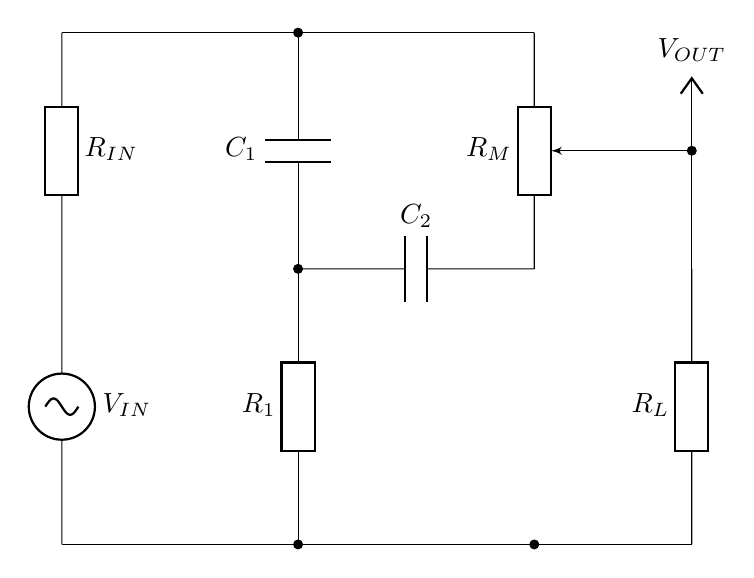
\begin{tikzpicture}
	\draw (1, 7) to[sinusoidal voltage source, l=$V_{IN}$] (1, 3.5);

	\draw (1, 10) to[european resistor, l=$R_{IN}$] (1, 7);
	\draw (4, 7) to[european resistor, l_=$R_1$] (4, 3.5);
	\draw (9, 7) to[european resistor, l_=$R_L$] (9, 3.5);

	\draw (7, 10) to[european potentiometer, l_=$R_M$] (7, 7);

	\draw (4, 7) to[capacitor, l=$C_1$] (4, 10);
	\draw (4, 7) to[capacitor, l=$C_2$] (7, 7);

	\draw (1, 10) -| (4, 10);
	\draw (9, 3.5) -- (1, 3.5);
	\draw (7, 10) -- (4, 10);
	\draw (7.5, 8.5) -- (9, 8.5) -- (9, 7);
	\draw (9, 9) -- (9, 8.5);

	\node[vcc] at (9, 9) {$V_{OUT}$};
	\node[circ] at (4, 10) {};
	\node[circ] at (4, 3.5) {};
	\node[circ] at (4, 7) {};
	\node[circ] at (7, 3.5) {};	
	\node[circ] at (9, 8.5) {};

\end{tikzpicture}
\end{document}